\documentclass[12pt,a4paper,article,english,firamath]{nsi}
\pagestyle{empty}
\begin{document}
\titre{Secret Santa\ \scriptsize(solution)}
\classe{Euro 1\ere}
\maketitle

\subsubsection*{From 00:00 to 00:42}
Explain what is Secret Santa.
\begin{encadrecolore}{Answer}{UGLiRed}
    Secret Santa is a method which makes each person in a group choose another one to give a present to, so that everybody buys a present for someone and also gets one.
\end{encadrecolore}
\subsubsection*{From 01:22 to 01:36}
What are the two fundamental things for a perfect Secret Santa ?
\begin{encadrecolore}{Answer}{UGLiRed}
    \begin{enumerate}
        \item It should be anonymous : nobody should know who bought his or her present.
        \item It should be perfectly random : you should have the same probability of getting a present from each member of the group.
    \end{enumerate}
\end{encadrecolore}
\subsubsection*{From 01:44 to 02:03}
How does Hannah describe the "hat method" ?
\begin{encadrecolore}{Answer}{UGLiRed}
    Everybody writes his or her name on a piece of paper and puts it in a hat.
    Then each member of the group successively picks a paper and reads a name. If someone picks his or her own name, he or she puts the paper back in the hat, otherwise, he or she will have to offer a present to the person whose name's written on the paper.
\end{encadrecolore}
\subsubsection*{From 02:03 to 02:46}
What is the obvious problem with this method and what does the group have to do in this case ?
\begin{encadrecolore}{Answer}{UGLiRed}
    If the last person's left with his or her own paper, there's nothing to do but start over.
\end{encadrecolore}
Why is there also an anonymity violation if the person before the last one pulls his or her name ?
\begin{encadrecolore}{Answer}{UGLiRed}
    Because in this case, he or she must take the only other remaining paper and everybody knows that the last person will get his or hers.
\end{encadrecolore}
\subsubsection*{From 02:46 to 10:59}
\picright{0.25}{img/tree_santa3_sol}{
    Despite of anonymity issues, let's see how  Secret Santa works with 3 persons.\\

    Complete this probability tree.\\

    When the method works, can we say is it completely random ?\\
    Justify your answer.}

\begin{encadrecolore}{Answer}{UGLiRed}
    No it is not, because for example, when the method works A it twice likely to buy for C than for B.
\end{encadrecolore}
\subsubsection*{From 11:00 till the end}
Explain what's the right way to organize a Secret Santa.
\begin{encadrecolore}{Answer}{UGLiRed}
\begin{itemize}
    \item Take as many cards as the number of people and write "You are number i" at the top and "You are buying for i" the bottom of each ($i$ starting from one to $n$, $n$ being the number of people). 
    \item Lay them face down and shuffle them.
    \item Cut them all up in the middle.
    \item Shift the tops along by one.
    \item Everybody take the two corresponding parts and find what's his or her number and who he or she is buying for.
\end{itemize}
\end{encadrecolore}
\subsection*{Bonus}

What's a derangement ?
\begin{encadrecolore}{Answer}{UGLiRed}
    A derangement is a permutation in which no object retains its original position.
\end{encadrecolore}

Complete the following tree for a "hat method" with 4 person.
\begin{center}
    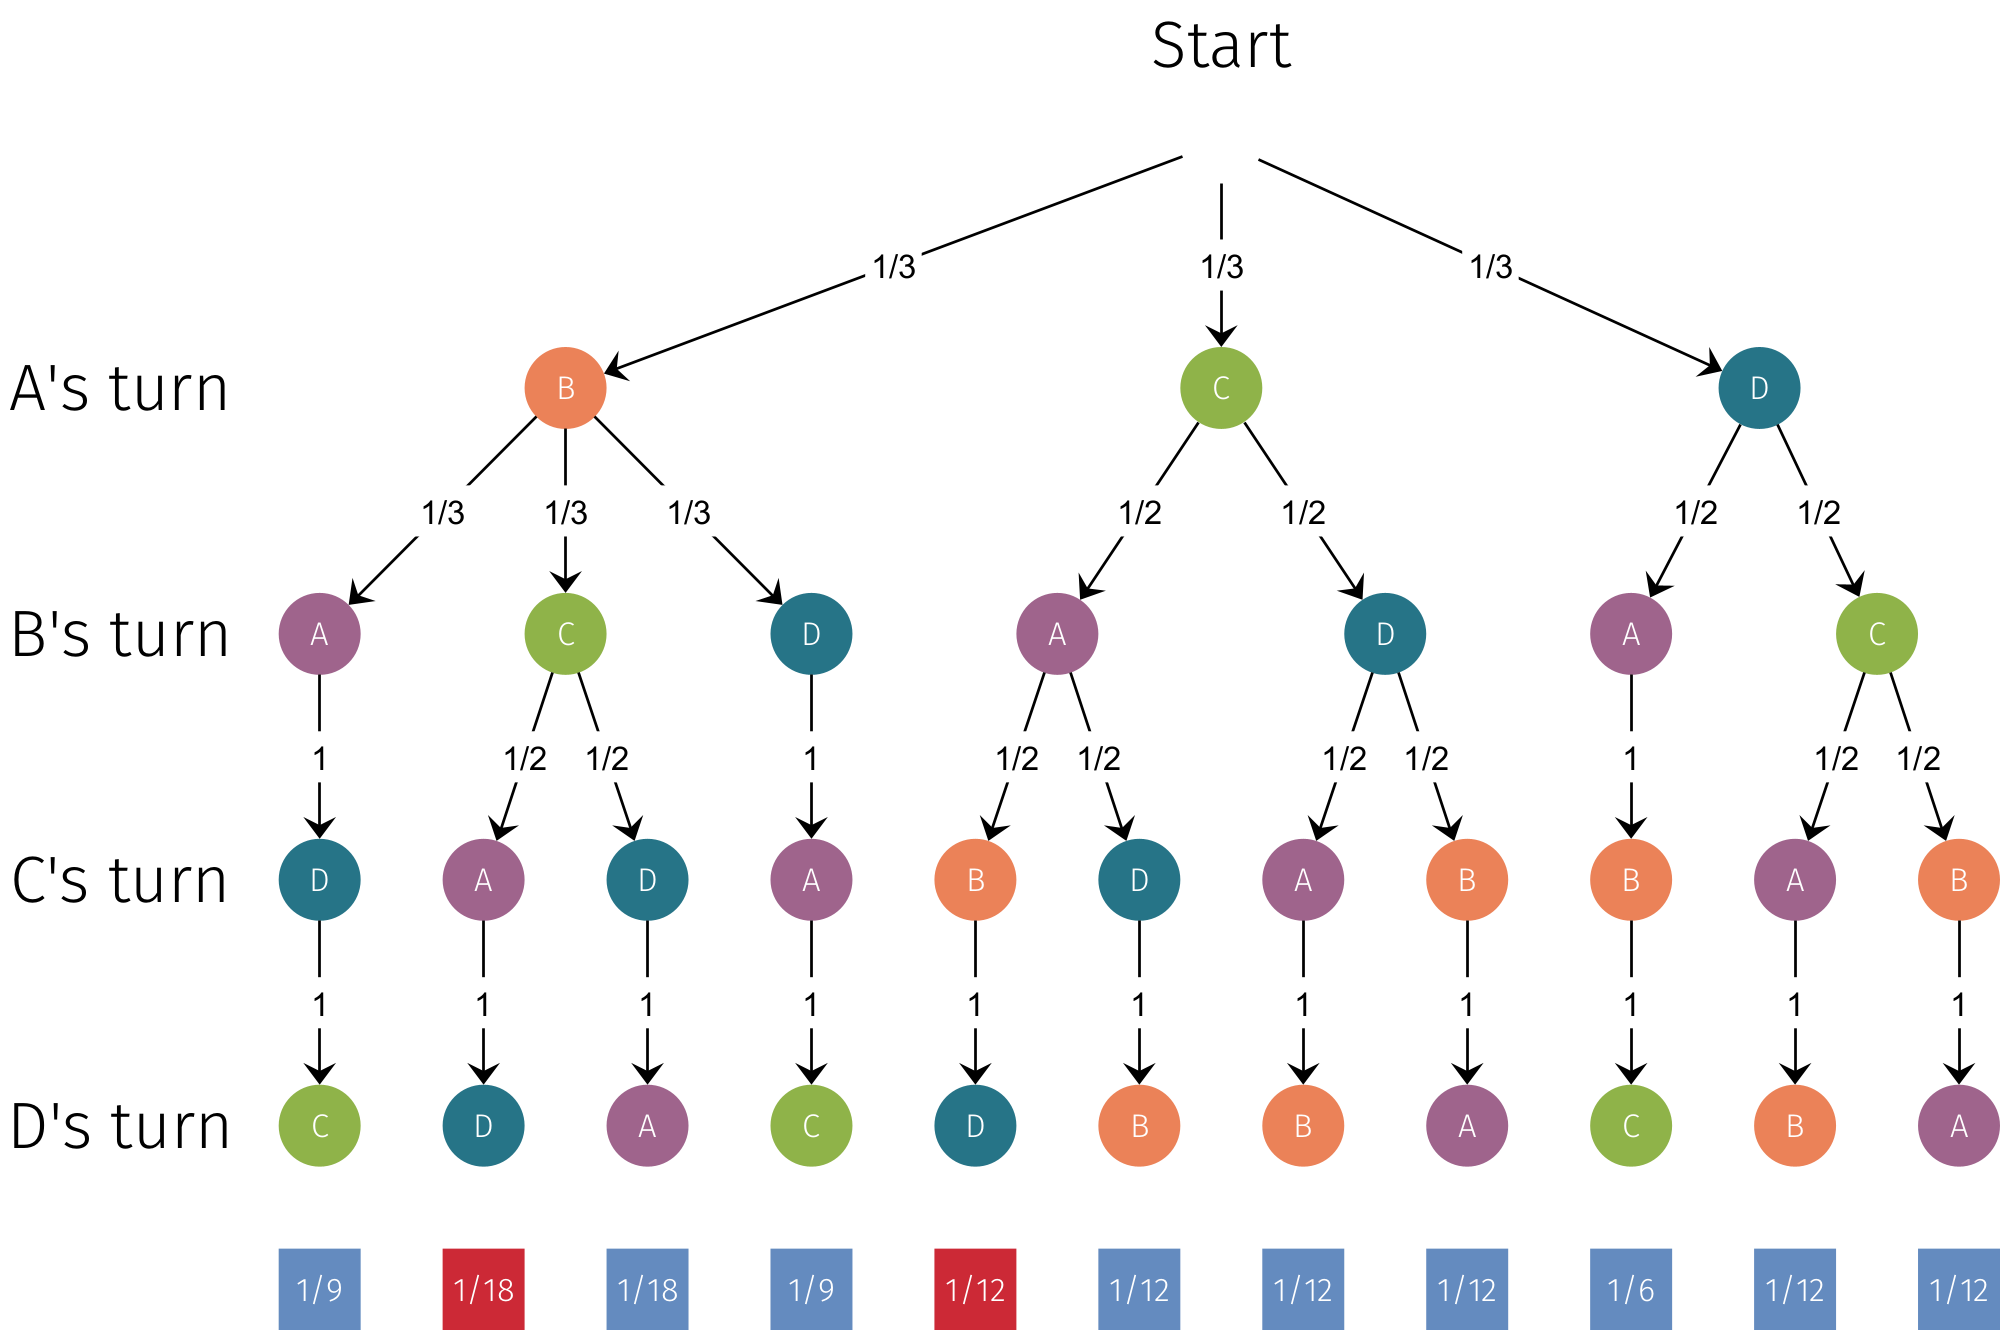
\includegraphics[width=13cm]{img/tree_santa4_sol.png}
\end{center}
What's the probability of a failure ?
\begin{encadrecolore}{Answer}{UGLiRed}
    It is $\frac{1}{18}+\frac{1}{12}=\frac{5}{36}\simeq 8.33\%$.
\end{encadrecolore}





\end{document}